\documentclass[a4paper]{article}
\usepackage{graphicx}

\begin{document}
\title{The TraGit DuckTale}
\author{F.dev}
\maketitle

\section*{Kapitel 1}
Det var en gång en badanka som heter Anki och en programmerare som heter Silas.
Klockan var efter midnatt och programmeraren brottades med en synnerligen svåridentifierad bug.

\begin{center}
	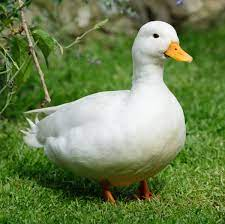
\includegraphics[scale=0.3]{duck.jpeg}
\end{center}

Han skulle lära sig Git, men det blev helt plötsligt väldigt svårt. Kanske han ska söka efter andra inlärnings-källor?

\section*{Kapitel 2}
Sökandet verkade totalt lönlöst. I sin desperation fick programmeraren syn på Anki.
``Varför funkar det inte?!'' utbrast programmeraren, till ingen annan än badankan som stod så ensam på skrivbordet.
Anki tittade djupt in i hens ögon, men sade inte ett ord. Medveten om att ingen kunde döma, började programmeraren förklara koden, steg för steg, med en detaljrikhet och inlevelse inte påträffad sedan Euclides Elementa!

\section*{Kapitel 3}
Bland allt svett och alla tårar som samlats på golvet fick Anki flyt. Då hände det! Programmeraren kom till slutet av filen och såg där:

\texttt{main}

Inga parenteser. Programmet började inte ens vid körning. Totalt chanslös att utföra ens den enklaste operationen. Med en djup suck av lättnad lade hen till parenteserna, och programmet kördes perfekt.

\end{document}
